%! TEX program = pdflatex
\documentclass[arbeit=studie,oneside,BCOR=12mm]{ArbeitRST}
\usepackage{amsmath} 
\usepackage{afterpage}
\usepackage{placeins}
\usepackage{algorithm}
\usepackage{algpseudocode}
\hypersetup{
    unicode=false,          % non-Latin characters in Acrobat’s bookmarks
    pdftoolbar=true,        % show Acrobat’s toolbar?
    pdfmenubar=true,        % show Acrobat’s menu?
    pdffitwindow=false,     % window fit to page when opened
    pdfstartview={FitH},    % fits the width of the page to the window
    pdftitle={Verbessung der Spurerkennung und -verfolgung autonomer Modellfahrzeuge}, % title
    pdfauthor={James Vero Asghar},     % author
    pdfsubject={Subject},   % subject of the document
    pdfcreator={James Vero Asghar},   % creator of the document
    pdfproducer={Producer}, % producer of the document
    pdfkeywords={stanley controller} {sliding window method} {model cars}, % list of keywords
    pdfnewwindow=true,      % links in new window
    colorlinks=true,        % false: boxed links; true: colored links
    linkcolor=blue,         % color of internal links (change box color with linkbordercolor)
    citecolor=green,        % color of links to bibliography
    filecolor=magenta,      % color of file links
    urlcolor=cyan           % color of external links
}
\setlength{\parindent}{0ex}
\setlength{\parskip}{2ex}

% Entfernt die farbigen Markierungen - bitte Druckversion mit dieser Option kompilieren
%\hypersetup{hidelinks}

\graphicspath{{./photos}}

\begin{document}

% Titelseite
% ==========

% Name des Verfassers
\author{James Vero Asghar}

% Geburtsort
\geburtsort{Austin, Texas, Vereignete Staaten}

% Geburtsdatum
\geburtsdatum{3. Dezember 1997}

% Titel der Arbeit
\title{Verbesserung der Spurerkennung und -verfolgung autonomer Modellfahrzeuge}

% Untertitel
\subtitle{}

% Angabe der Betreuer
\betreuer{Dr.-Ing. Carsten Knoll}
\betreuer{M.Sc. Paul Auerbach}

% Datum der Einreichung
\date{2. Februar 2222}


% Zunächst für das Vorgeplänkel römische Seitenzahlen und einfacher Seitenstil
% ============================================================================
\pagenumbering{Roman}
\pagestyle{plain}


% Titelseite erstellen
\maketitle


% Selbstständigkeitserklärung
% ===========================

% Selbstständigkeitserklärung erstellen
\selbststaendigkeitserklaerung


% Kurzfassung / Abstract
% ======================
\kurzfassung{An dieser Stelle fügen Sie bitte eine deutsche Kurzfassung ein.}
{At the Connected Robotics Lab (CoRoLa) research group at the Barkhausen
Institut, a demonstration using remote controlled 2 axis vehicles was
developed. The demonstration is currently in use in order to model
communications between vehicles similar to an Internet of Things (IoT) network.

In order to better model the complexities of a real world system a nonlinear
control algorithm was introduced to the system in order to more accurately
control the vehicles. The Stanley Controller is a nonlinear controller
developed for use with the lateral control of 2 axis vehicles in mind. As input
to the controller, a fisheye camera was used to create images of road. These
images were then digitally processed to find the yellow line for the vehicles
to follow.}


% Inhaltsverzeichnis
% ==================
\tableofcontents

\chapter{Einführung}

At the Connected Robotics Lab (CoRoLa) research group at the Barkhausen
Institut, a demonstration using remote controlled two axle vehicles was
developed. The demonstration is currently in use in order to model
communications between vehicles similar to an Internet of Things (IoT) network.

Due to issues regarding low forward velocity and robustness of the current
vehicle controller, it was proposed to implement a new 

In order to achieve the goals stated above, creation of an image processing
pipeline and implementation of the Stanley controller are proposed.

\chapter{Regelalgorithmus}

\section{Stanley-Regler}

Der Stanley-Regler ist ein nichtlinearer Regelungsalgorithmus, der 2005 von
der Stanford University entwickelt wurde, um ein zweiachsiges Fahrzeug nur
anhand der Ausrichtung des Fahrzeugs relativ zur Bahn und der Querabweichung der zu verfolgenden Bahn zu
steuern. Der Algorithmus hat sich für das kinematische Modell eines
zweiachsigen Fahrzeugs als asymptotisch global stabil erwiesen.

Der Stanley-Regler ist ein Bahnfolgeregler anstelle eines
Trajektorienfolgereglers. Als Querregler soll er das Fahrzeug auf der Bahn
halten, hat aber keinen Einfluss auf die Vorw"artsgeschwindigkeit. Dieser
Ansatz ermöglicht eine flexible Wahl der Fahrzeuggeschwindigkeit, die unter
Berücksichtigung dynamischer Effekte nach Bedarf für eine bestimmte Anwendung
gewählt werden kann. 

Der Stanley-Regler wird mathematisch durch die folgende Gleichung beschrieben:
\begin{equation} 
  u = \theta - \theta_d + \arctan\left(\frac{ke_{V}}{v}\right).
  \label{eq:Stanley-Regler} 
\end{equation}
Dabei ist $u$ den Reglerausgang, $\theta$ die aktuelle Ausrichtung des Fahrzeugs,
$\theta_d$ die Kursausrichtung, $k$ ein Skalierungsfaktor, $v$ die
Geschwindigkeit des Fahrzeugs und $e_{V}$ die Querabweichung vom Mittelpunkt
der Vorderachse des Fahrzeugs zum Kurs.

Der Stanley-Regler besteht aus zwei Komponenten: einer Komponente, die die
Querabweichung des Fahrzeugs vom Kurs behandelt, und einer Komponente, die die
Differenz zwischen der Ausrichtung des Fahrzeugs und der des Kurses behandelt.
Die erste Komponente wird durch $\arctan(\frac{ke_{V}}{v})$ dargestellt und
steuert den Lenkwinkel so, dass er sich auf den Kurs zubewegt, wenn sich das
Fahrzeug weiter von ihm entfernt. Die zweite Komponente, dargestellt durch
$\theta_d - \theta$, steuert den Lenkwinkel so, dass er parallel zum zu
verfolgenden Kurs bleibt. Zusammen bewirken diese beiden Komponenten, dass
das Fahrzeug auf den gewünschten Kurs gelenkt wird.


\subsection{Kleinsignalverhalten}


Um das Verhalten des Stanley-Reglers besser zu verstehen, wird der Regler um
den Punkt $\left(x_V, \theta_d\right) = \left(0, 0\right)$
linearisiert, was zu folgender Gleichung führt: 
\begin{equation} \bar{u} \approx \bar{\theta} + \frac{k}{v}e_{V}. 
    \label{eq:linearer Stanley-Regler}
\end{equation}

Die sich daraus ergebende Gleichung \eqref{eq:linearer Stanley-Regler} hat die
Form eines PID-Reglers (Proportional-, Integral- und Derivativ-Regler), der nur
P- und D-Komponenten hat. Die P-Komponente wird durch \(\frac{k}{v}e_{V}\)
dargestellt. Da die Vorwärtsgeschwindigkeit des Fahrzeugs als konstant
angenommen wird, besteht eine Proportionalität zwischen den Ableitungen von
\(e_{V}\) nach Zeit und Raum. Die Ableitung von \(e_{V}\) nach dem Raum ist
\(\theta\). Daher ist \(\theta\) die D-Komponente des linearisierten
Stanley-Reglers.

Folglich ist das Verhalten des Stanley-Reglers für kleine Eingangssignale
ähnlich wie das eines PD-Reglers mit dem Fehlerterm \(e_{V}\). 


\subsection{Gro{\ss}signalverhalten}

Bei großen Signalen wird der Stanley-Regler durch das Verhalten der
\(arctan\)-Funktion sowie durch die zyklische Natur der Ausrichtung
\(\theta\) dominiert. Die Funktion \(arctan\) ist auf einen Wert zwischen
-90 und 90 Grad begrenzt und ist glatt. Die Ausrichtung ist ebenfalls auf den
vorderen Halbkreis des Fahrzeugsichtfelds bzw. -90 und 90 Grad begrenzt, da davon ausgegangen wird,
dass sich das Fahrzeug in eine Richtung bewegt. Zusammen begrenzen diese
Komponenten den Lenkwinkel des Fahrzeugs.


%Beim Umgang mit großen Signalen wird das Verhalten des Stanley-Reglers
%hauptsächlich von zwei Faktoren beeinflusst: der zyklischen Natur der
%Ausrichtung \(\theta\) und der \(arctan(...)\)-Funktion. Die Funktion
%\(arctan(...)\) ist eine glatte Funktion, die auf einen Bereich zwischen -90
%und 90 Grad begrenzt ist. Andererseits ist die Ausrichtung auf den vorderen
%Halbkreis beschränkt, der zwischen -90 und 90 Grad liegt, da davon ausgegangen
%wird, dass sich das Fahrzeug in eine Richtung bewegt. Diese beiden Faktoren
%wirken also zusammen, um den Lenkeinschlag des Fahrzeugs zu begrenzen und zu
%verhindern, dass er zu groß wird.

\section{Simulation}


Um ein besseres Verständnis für das Verhalten des Stanley-Reglers in einem
Modellfahrzeug zu gewinnen, habe ich eine Simulation des
Regelkreises durchgeführt. Die Simulation umfasst drei Hauptkomponenten: den
Kurs, dem das Fahrzeug folgen muss, den Stanley-Regler und das Fahrzeugmodell.
Zur Untersuchung der Zeitreihendaten des zweiachsigen Fahrzeugs in der
Simulation wurde ein Differentialgleichungslöser eingesetzt.

Der Kurs, dem das Fahrzeug folgen muss, ist eine virtuelle Darstellung der
realen Strecke, die das Fahrzeug durchfahren wird. Eine visuelle
Darstellung der Fahrbahn findet sich in Abb. \ref{fahrbahn}. In der Simulation wird der
Kurs durch die folgende kontinuierliche statische Funktion definiert:
\begin{equation} 
  (x, y, h) = f(t, t_f), 
\end{equation} 
wobei $t$ und $t_f$ die Eingangsparameter Zeit bzw. Simulationsdauer sind
und $(x, y, h)$ die kartesischen Koordinaten des Pfadpunkts und die
entsprechende Ausrichtung an diesem Punkt darstellt. Diese Funktion wird für
eine beliebige Anzahl von $t$-Werten diskretisiert, um eine Liste von $(x, y,
theta)$-Werten zu erzeugen. Der Differentialgleichungslöser bezieht den
Stanley-Controller und das Fahrzeugmodell ein, um die Zeitreihen des
zweiachsigen Fahrzeugs unter Verwendung dieser Liste als Eingabe zu
analysieren.

\begin{figure}[h]
    \centering
    \includegraphics[scale=0.5]{Fahrbahn}
    \caption{Fahrbahn}
    \label{fahrbahn}
\end{figure}


Das verwendete Fahrzeugmodell ist das Modell eines Hinterachsfahrzeugs. Dieses
Modell wird durch die folgende nichtlineare Zustandsraumdarstellung
dargestellt: 
\begin{gather} 
  \dot{x} = v \cos(\theta) \\ 
  \dot{y} = v \sin(\theta) \\ 
  \dot{\theta} = \frac{v}{l}\tan(\varphi) \\
  \dot{\varphi} = \frac{\left(\delta-u\right)}{T}. 
\end{gather}

Die Zustandsvariablen des Modells sind $x_H$, $y_H$, $\phi$ und $\theta$, wobei
$x_H$ und $y_H$ die kartesischen Koordinaten des Mittelpunkts der Hinterachse
sind und $\theta$ die Ausrichtung des Fahrzeugs ist. $\varphi$ ist der
Lenkwinkel des Fahrzeugs. Die Eingangsgrößen des Modells sind $v$ und
$\varphi$, wobei $v$ die Geschwindigkeit des Fahrzeugs und $\varphi$ der
Lenkwinkel ist. Der Lenkwinkel $\varphi$ ist selbst ein dynamisches System, das
durch eine lineare Differentialgleichung erster Ordnung mit der
konfigurierbaren Zeitkonstante $T$ dargestellt wird. $l$ ist der Abstand
zwischen dem Hinterradachse und dem Vorderradachse.  Das Verhalten des
Stanley-Reglers bei dynamischen Einflüssen auf den Lenkwinkel ist von großer
Bedeutung, da die globale asymptotische Stabilität des Reglers nur für das
kinematische Zweiachsmodell nachgewiesen wurde.

Da der Stanley-Regler für die Querabweichung den Mittelpunkt der Vorderachse
benötigt, muss dieser aus der Hinterachse berechnet werden. Der Mittelpunkt der
Vorderachse wird aus den Zustandsvariablen durch die folgende statische
Funktion berechnet: 
\begin{gather}
  \underline{p}_H := 
  \begin{bmatrix}
    x_H & y_H
  \end{bmatrix}^T \\
  \underline{p}_V := 
  \begin{bmatrix}
    x_V & y_V
  \end{bmatrix}^T
  \label{eq:Rear Axle and Front Axle}
\end{gather}
\begin{equation}
  \underline{p}_V = \underline{p}_H + l 
  \begin{bmatrix}
    \cos(\theta + \pi/2) \\ 
    \sin(\theta + \pi/2),
  \end{bmatrix}
  \label{eq:Transformation from Rear Axle to Front Axle}
\end{equation}
wobei $x_V$ und $y_V$ die kartesischen Koordinaten dieses Vorderradachsemittelpunkts sind.
$\underline{p}_V$ und $\underline{p}_H$ sind die Positionsvektoren des
Hinterrad- und Vorderradachsemittelpunkts.

Wie bereits erwähnt, besteht der Stanley-Regler aus mehreren Teilen, die
getrennt voneinander berechnet werden k"onnen. Die Ausrichtung $\theta$ ist eine
Zustandsvariable, daher ist sie immer verfügbar. Um die Querabweichung und die
Kursrichtung zu berechnen, muss der richtige Bahnpunkt gewählt werden. Der
Stanley-Regler verwendet den nächstliegenden Bahnpunkt vom
Vorderachsmittelpunkt des Fahrzeugs, um die Ausrichtung des Kurses $\theta_d$
und die aktuelle Querabweichung $e_{V}$ zu bestimmen. Für die Simulation wird
dies bestimmt, indem der Punkt mit dem geringsten Abstand zum
Vorderachsmittelpunkt $\delta\underline{x}$ gefunden wird. An diesem Punkt wird
dann die Ausrichtung des Kurses ermittelt. Das Skalarprodukt zwischen dem
Vektor senkrecht zur Fahrzeugausrichtung $\underline{x}_{\perp}$ und dem Vektor
vom Pfadpunkt zur Fahrzeugvorderachse $\delta\underline{x}$ ist die
Querabweichung $e_{V}$. Zur Verdeutlichung ist in ABBILDUNG eine visuelle
Darstellung dieser beiden Vektoren und ihres Skalarprodukts abgebildet. Dieser
Algorithmus wird in folgende Algorithmus dargestellt. \\

\begin{figure}[h]
    \centering
    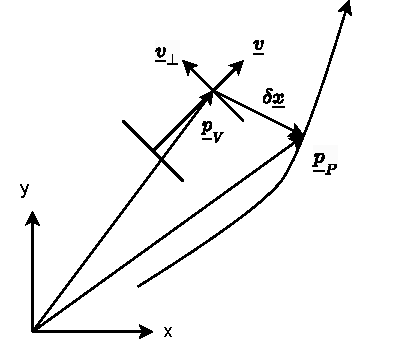
\includegraphics{dot_product}
    \caption{Berechnung von Querabweichung}
    \label{algorithm}
\end{figure}

\begin{algorithm}
  \caption{Berechnung von Querabweichung}
  \label{alg:quer}
  \begin{algorithmic}
    \State $\underline{v}_{\perp} \gets \left[-\cos(\theta + \pi/2),  -\sin(\theta + \pi/2)\right]^T$
    \State $\Delta\underline{x} \gets \underline{p}_V - \underline{p}_P$
    \State $\delta\underline{x} \gets \min \left{ || \Delta\underline{x} ||_2 \right}$
    \State $\theta_d \gets \arctan\left(\frac{\frac{d}{dy}\delta\underline{x}}{\frac{d}{dx}\delta\underline{x}}\right)$
    \State $e_{V} \gets \delta\underline{x} \cdot \underline{v}_{\perp}$
  \end{algorithmic}
\end{algorithm}

Der Kurs und die Querabweichung werden dann in den Stanley-Regler eingegeben,
und der Ausgang des Reglers wird in das Fahrzeugmodell eingespeist. Ein
Übersichtsdiagramm des Regelkreises ist in ABBILDUNG dargestellt.

\begin{figure}[h]
    \centering
    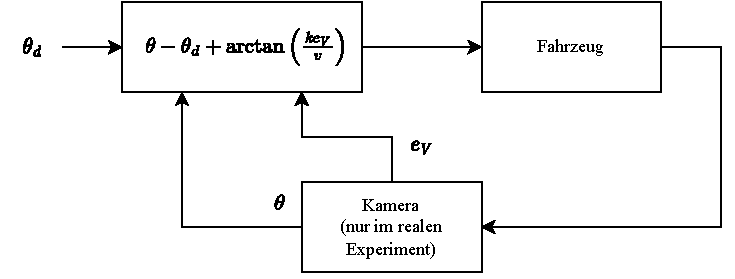
\includegraphics{control_loop}
    \caption{Regelkreis}
    \label{control_loop}
\end{figure}

Der Stanley-Regler arbeitet mit zeitkontinuierlichen Signalen, die sich von den
vom \glqq echten\grqq Fahrzeug verwendeten zeitdiskreten Signalen
unterscheiden. Das Fahrzeug nimmt Bilder mit einer festen Abtastfrequenz auf,
die von der Pipeline verarbeitet werden, bevor sie in den Regler eingespeist
werden. Um dieses Verhalten zu simulieren, wird ein Speicher in den Simulator
eingebaut, um die Ausrichtung und die Querabweichung zu speichern. Der
Stanley-Regler verwendet dann diese zwischengespeicherten Werte für eine
bestimmte Dauer. Dieser Speicher-Ansatz ahmt das Verhalten eines Halteglieds
nullter Ordnung nach, und die Ausgabe dieses Haltegliedes wird anschließend in
den Stanley-Regler eingespeist. Dieser Simulationsansatz ermöglicht die
Untersuchung des Fahrzeugverhaltens für verschiedene Abtastfrequenzen. Von
besonderer Bedeutung ist die Stablit"at des Regelkreises mit verschiedenen
Abtastfrequenzen. Der Vergleich der Simulationsergebnisse bei
verschiedenen Abtastfrequenzen ist in Abb. \ref{sampling} dargestellt. 

\begin{figure}[h]
    \centering
    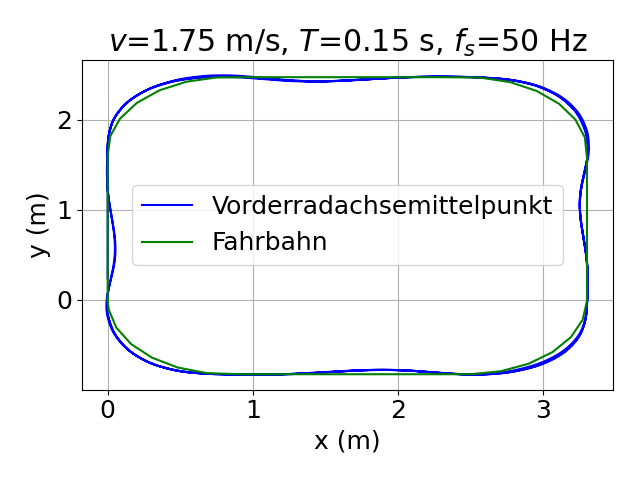
\includegraphics[scale=0.47]{50Hz}
    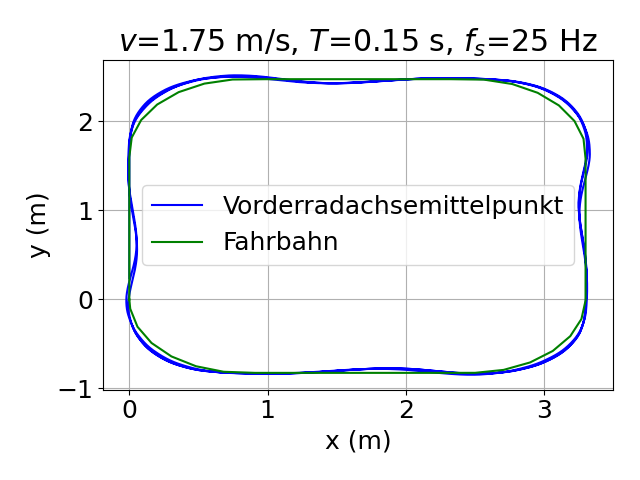
\includegraphics[scale=0.47]{25Hz}
    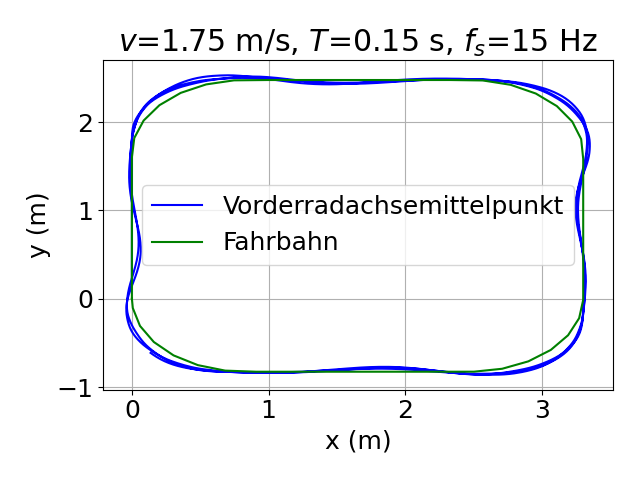
\includegraphics[scale=0.47]{15Hz}
    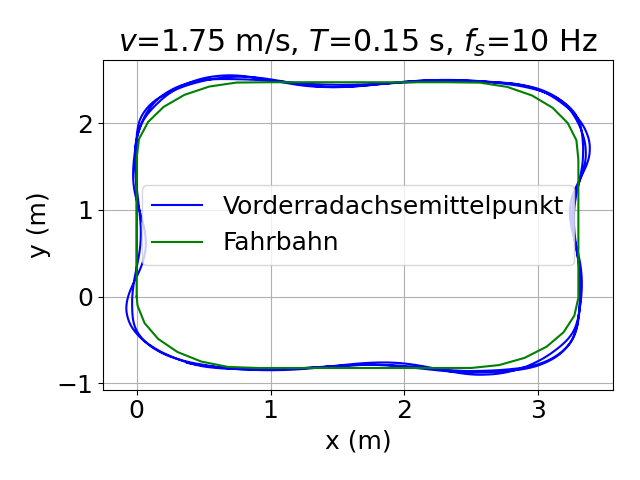
\includegraphics[scale=0.47]{10Hz}
    \caption{Abtastfrequenzen}
    \label{sampling}
\end{figure}

Wie in Abb. \ref{sampling} dargestellt, wird der Stanley-Regler durch die Abtastfrequenz
beeinflusst, wobei bei niedrigeren Frequenzen ein deutlicher Effekt zu
beobachten ist. Oberhalb eines bestimmten Schwellenwerts von 15 Hz scheint das
Verhalten des Fahrzeugs jedoch nicht wesentlich durch die Abtastfrequenz
beeinflusst zu werden. 

Die Simulation wurde dann für eine ausgewählte Zeitspanne durchgeführt. 



\chapter{Bildverarbeitung}
\section{Kamera-Kalibrierung}

Am Anfang der Bildverarbeitungspipeline steht die Kamerakalibrierung. Für die
CoRoLa Car Platform wurde eine Fischaugenkamera im Gegensatz zu einer
geradlinigen Kamera gewählt. Der Vorteil einer Fischaugenkamera ergibt sich aus
ihrem größeren Blickwinkel im Vergleich zu einer geradlinigen Kamera. Eine
Fischaugenkamera hat eine tonnenförmige Verzeichnung,
wodurch gerade Linien gekrümmt werden. Die Krümmung dieser Linien hängt von
ihrem radialen Abstand vom Bildmittelpunkt ab. Ein Beispiel ist in Abb.
\ref{barrel} zu sehen. Diese Verzeichnung kann mit Hilfe der Software durch die
sogenannte Kamerakalibrierung kompensiert werden. \\

\begin{figure}[h]
    \centering
    \fbox{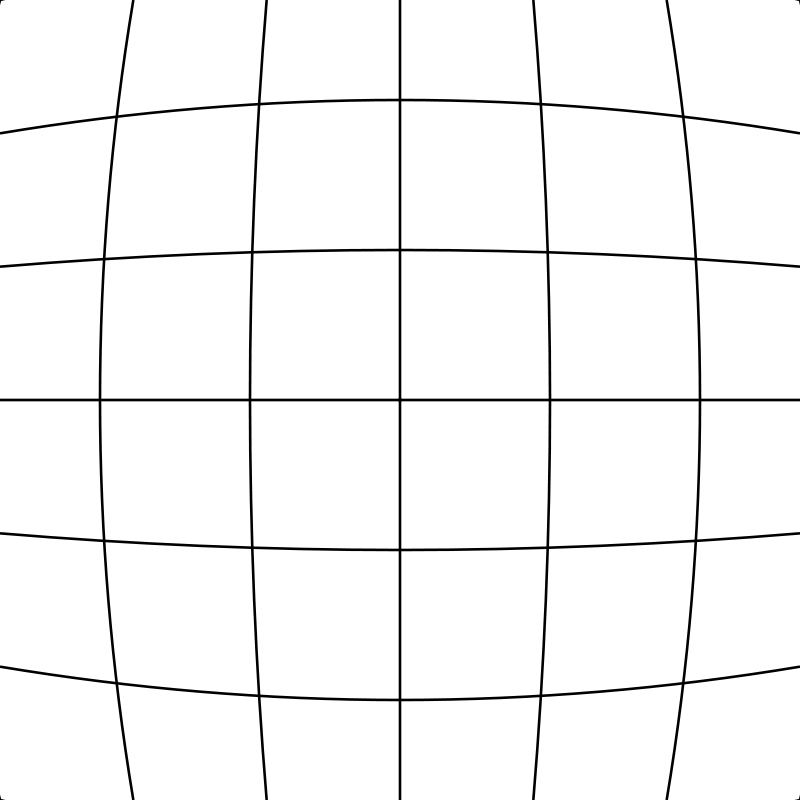
\includegraphics[scale=0.175]{Barrel_distortion}}
    \caption{Verzeichnung}
    \label{barrel}
\end{figure}

Die Kamerakalibrierung wird verwendet, um die extrinsischen und intrinsischen
Parameter einer Kamera n"ahrungsweise zu bestimmen. Eine kalibrierte Kamera ermöglicht es,
3-D-Informationen aus einem 2-D-Bild zu gewinnen. Die intrinsischen Parameter
einer Kamera werden häufig durch die folgende 3x3-Matrix dargestellt:
\begin{equation} 
    K = 
    \begin{bmatrix} 
        f_x & 0 & c_x\\ 
        0 & f_y & c_y\\ 
        0 & 0 & 1
    \end{bmatrix}, 
\end{equation} 
wobei $f_x$ und $f_y$ die Brennweiten der Kamera in Pixeln in den
Richtungen $x$ und $y$ und $c_x$ und $c_y$ die Koordinaten des Bildmittelpunkts
sind. Die extrinsischen Parameter werden häufig durch die folgende Matrix
dargestellt: 
\begin{equation}
    \begin{bmatrix} R & T \end{bmatrix}. 
\end{equation} 
Dabei ist $R$ die Rotationsmatrix der Kamera in Bezug auf das Laborsystem (?) und $T$
der Positionsspaltenvektor des Ursprungs des Laborsystems, ausgedrückt in den
Koordinaten des Kamerabildes. Die Kameramatrix $M$ ist die Abbildung von
den Weltkoordinaten auf Pixelkoordinaten, die durch die
Matrix-Matrix-Multiplikation dargestellt wird, 
\begin{equation} 
    M = K 
    \begin{bmatrix} 
        R & T
    \end{bmatrix}. 
\end{equation} 
Durch Rekonstruieren der $M$-Matrix mit Hilfe von Software kann das verzerrte
Bild wieder in das Weltbild "uberf"uhrt werden, wodurch gekrümmte Linien gerade
werden. \\

\begin{figure}[h]
    \centering
    \fbox{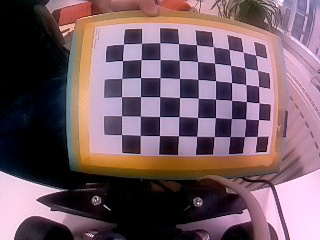
\includegraphics[scale=0.75]{before_calibration_checkerboard}}
    \fbox{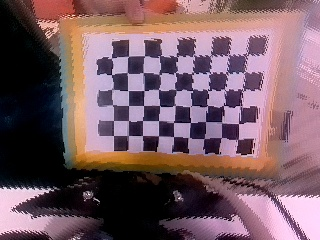
\includegraphics[scale=0.75]{after_calibration_checkerboard}}
    \caption{Calibrated Images.}
    \label{checkerboards}
\end{figure}

Eine Kamera wird anhand einer Sammlung von Fotos mit bekannten geraden Linien
kalibriert. In der Regel wird eine Reihe von Schachbrettbildern mit bekannten
Dimensionen verwendet. Danach werden Fotos des Schachbretts in verschiedenen
Winkeln und in verschiedenen Positionen relativ zu Kamera aufgenommen. Diese Bilderserie
wird dann in den Algorithmus zur Kamerakalibrierung eingespeist, der zunächst
die Positionen der Schachbrettfelder und der sie verbindenden Linien bestimmt.
Anschließend gleicht der Algorithmus anhand des Modells einer Fischaugenkamera
die Verzeichnung aus. Wie in Abb. \ref{checkerboards} zu sehen, werden
beispielsweise die gekrümmten Linien des Schachbretts nach der Kalibrierung
wieder gerade gemacht. Die Anzahl der benötigten Bilder hängt von der
jeweiligen Kamera ab, eine große Sammlung von Fotos führt jedoch zu einer
genaueren Annäherung an die Parameter. (Zitat OPENCV) Die Verwendung von
Bildern mit einer höheren Auflösung führt ebenfalls zu genaueren Parametern.
(Zitat OPENCV/BLOG) Die angenäherten Parameter sind jedoch nur für die
Kalibrierung von Bildern sind g"ultig, die mit der gleichen Auflösung aufgenommen
wurden wie die für die Kalibrierung verwendeten Bilder. Um die Kameramatrix für
Bilder mit einer niedrigeren Auflösung zu verwenden, muss die intrinsische
Kameramatrix $K$ mit der folgenden Formel skaliert werden: 
\begin{equation} 
    K_n = k K, 
\end{equation} 
wobei $k$ ein skalarer Wert ist, der den Skalierungsfaktor darstellt. Da es
sich bei der intrinsischen Kameramatrix um eine affine Abbildung handelt, muss
der Wert bei $K_{n3, 3}$ auf 1 gesetzt werden. Die resultierende intrinsische
Kameramatrix funktioniert bei kleineren Auflösungen, die dem Seitenverhältnis
der für die Kalibrierung verwendeten Bilder gleich sind. 


\iffalse
Allerdings wurde
beobachtet, dass bei einem zu großen Auflösungsunterschied Verzeichnungen
wieder in das Bild eingefügt werden. In ABBILDUNG ist links das Originalbild zu
sehen, das mittlere Bild wurde mit Bildern von 900p kalibriert und das rechte
Bild mit Bildern von 240p. Wie man sieht, wird das Lineal im rechten Bild
gerade, während es im mittleren Bild gekrümmt bleibt.
\fi

Ein Nachteil der Kamerakalibrierung ist, dass jedes kalibrierte Bild eine
geringere Auflösung hat als das Originalbild. Dies ist eine Folge des
Kalibrierungsprozesses, da dieser einen Teil des Bildes verzerrt,
insbesondere die Pixel in den Ecken des Bildes. Daher werden diese Pixel beim
Kalibrierungsprozess aus dem resultierenden Bild entfernt. Um das Bild in
seiner ursprünglichen Auflösung zu rekonstruieren, wird eine Interpolation
verwendet. Die Interpolation liefert jedoch ein unschärferes Bild als das
Original. Um dies zu kompensieren, empfiehlt es sich, eine Kamera mit
hochauflösenden Bildern zu kalibrieren und dann Bilder mit dieser Auflösung
aufzunehmen. Anstatt den Interpolator zu verwenden, verkleinern Sie die Bilder
dann auf eine Auflösung, die für die jeweilige Anwendung erforderlich ist.  Das
Ergebnis ist ein genaueres Bild ohne Unschärfe. Leider ist dieser Prozess sehr
rechenintensiv, und es wurde beschlossen, nur die Bilder aus dem Interpolator
zu verwenden, um die Rechenleistung der Pipeline zu erhöhen.

Ein weiterer Nachteil der Kamerakalibrierung ist, dass sich der Mittelpunkt der
Kamera verschieben kann. Ein Beispiel dafür ist in Abb. \ref{shifted} zu sehen. Durch
manuelles Ändern von $c_x$ kann der Bildmittelpunkt wieder an seine
ursprüngliche Position verschoben werden. 

\begin{figure}[h]
    \centering
    \fbox{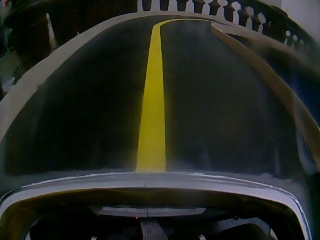
\includegraphics[scale=0.5]{orig_not_shifted}}
    \fbox{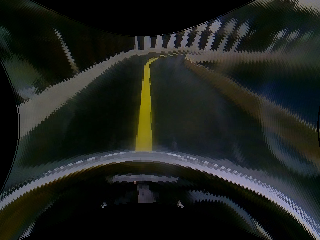
\includegraphics[scale=0.5]{cal_shifted}}
    \caption{Shifted Images.}
    \label{shifted}
\end{figure}

\section{\glqq Color Thresholding\grqq}

Als Nächstes folgt der Schritt des sogenannten "Color Thresholding". In dieser
Stufe werden alle Pixel aus dem Bild entfernt, die nicht zur Bahnlinie geh"oren.
In dieser Implementierung sind Farbe ausser Gelb ungew"unscht.

Zunächst wird das Bild von allen Pixeln ohne hohen Rotanteil gefiltert, da
Hellgelb im Rot-Grün-Blau-Farbraum (RGB) einen hohen Rotanteil hat.
Anschließend wird das Bild in den HSV-Farbraum (Hue, Saturation, Value engl. f"ur Farbwert, Sättigung und
Hellwert) umgewandelt. 

Im RGB-Farbraum ist reines Gelb so definiert, dass sowohl der rote als auch der
grüne Kanal gleich sind und der blaue Kanal auf Null gesetzt ist. Dies lässt
nur einen Freiheitsgrad für die Justierung der Pipeline zu.  Ein einziger
Freiheitsgrad führt zu Problemen bei der Abstimmung, da die Pipeline dadurch
weniger in der Lage ist, Störungen zu berücksichtigen. Unterschiedliche
Lichtverhältnisse oder reflektierende Oberflächen sind Beispiele für solche
Störungen.

Im HSV-Farbraum bestimmt der Farbwertkanal die Farbe, der Sättigungskanal die
Reinheit des Farbtons und der Wertekanal die Helligkeit des Farbtons. (MS ANNO)
Nach der Auswahl des Farbwerts, in diesem Fall Gelb, werden der Helligkeits-
und der Sättigungskanal verwendet, um den spezifischen Gelbton auszuwählen. Die
Verwendung dieser beiden Kanäle ermöglicht eine zuverlässigere Erkennung der
Farbe.

Um die gelbe Spur zu erkennen, filtert die Pipeline Farben außerhalb des gelben
Farbtonbereichs heraus und schneidet dann den unteren Teil des Helligkeits- und
Sättigungskanals ab. Das Ergebnis ist, dass nur reines Gelb im Bild übrig
bleibt. Die in der Pipeline verwendeten Werte für Gelb werden durch den
folgenden Bereich, TABLE, dargestellt.

Das Ergebnis dieser Stufe der Pipeline ist beispielsweise in Abb. \ref{color-thresholding}
dargestellt. Als Eingabe bekommt der Pipeline ein kalibriertes Bild und er gibt nur Pixel aus, die 
zur Bahnlinie geh"oren. \\

\begin{figure}[h]
    \centering
    \fbox{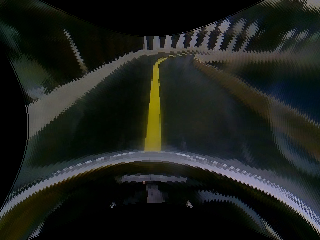
\includegraphics[scale=0.5]{calibrated}}
    \fbox{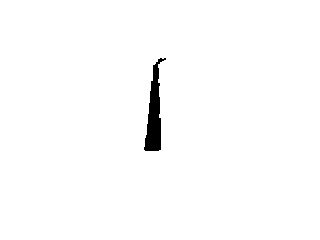
\includegraphics[scale=0.5]{thresholded}}
    \caption{Thresholded image.}
    \label{color-thresholding}
\end{figure}

\section{Perspektivtransformation}

Der dritte Teil der Bildverarbeitungspipeline ist die Perspektivtransformation. 
Das Kamera steht nicht senkrecht zur Bahn, sondern steht es winkelig zur Bahn

Wenn ein Bild mit einer am Fahrzeug montierten Kamera aufgenommen wird, ist die
Fahrbahn nicht rechteckig, sondern trapezförmig. Diese Perspektive
erfordert, dass alle Berechnungen bezüglich der Fahrspurlinie deren scheinbar abnehmende
Breite kompensieren müssen. Um dies zu vermeiden, wird eine
Perspektivtransformation durchgeführt. 

Bei der Perspektivtransformation wird eine Teilmenge eines Bildes beschnitten
und so angepasst, dass sie das gesamte Bild umfasst. Ein Beispiel ist in
Abb. \ref{roi-pt} dargestellt. Bei diesem Projekt ist die Form der Teilmenge des Bildes
ein Trapez. Mithilfe dieser Perspektivtransformation wird die trapezförmige
Form der Fahrbahnlinie in eine gerade Form korrigiert, wie in Abb. \ref{roi-pt}
dargestellt. \\

\begin{figure}[h]
    \centering
    \fbox{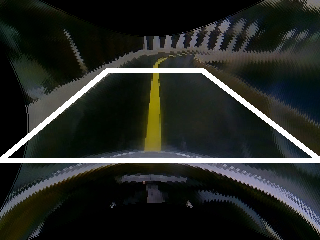
\includegraphics[scale=0.5]{roi.png}}
    \fbox{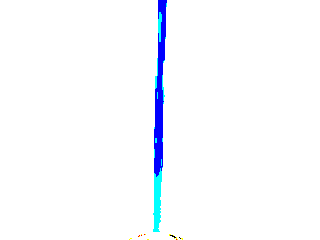
\includegraphics[scale=0.5]{perp_trans.png}}
    \caption{ROI, Inverted Perspective Trans.}
    \label{roi-pt}
\end{figure}

Eine Folge dieser neuen Perspektive ist, dass das resultierende Bild einer
2-D-Ebene der Strecke ähnelt. Die Perspektivtransformation vereinfacht auch die
weitere Bildverarbeitung, da alle Objekte außerhalb des Trapezes abgeschnitten
werden und nur die Spur übrig bleibt. Wie in Abb. \ref{roi-pt} zu sehen ist, führt die
Perspektivtransformation jedoch zu zusätzlichem Rauschen im Bild. Die durch die
Perspektivtransformation verursachte Scherung führt dazu, dass die Pixel des
Originalbildes gestreckt werden, wodurch das Bild mit Rauschen verunreinigt
wird. Daher ist es erforderlich, dass diese Stufe nach der
\glqq Color-Thresholding\grqq-Stufe erfolgt.

\section{Histogramm}

Nach der Perspektivtransformation wird ein Histogramm der schwarzen Pixel erstellt,
um den Startpunkt für die Gleitfenstermethode zu bestimmen. Die Anzahl der
weißen Pixel wird für jede Spalte des Bildes gezählt, und diese Zahlen werden
in einer Liste gespeichert. Es wird davon ausgegangen, dass die Spalten mit den
höchsten Zahlen Fahrspurinformationen enthalten, und der Index der Spalte mit
der höchsten Zahl wird als Startpunkt für die Gleitfenstermethode gewählt.
Dieser Schritt trägt dazu bei, die Berechnungszeit zu verkürzen, indem Teile
des Bildes herausgefiltert werden, die keine Fahrspurinformationen enthalten.
Eine visuelle Darstellung des Histogramms ist in Abb. \ref{hist} zu sehen. \\

\begin{figure}[h]
    \centering
    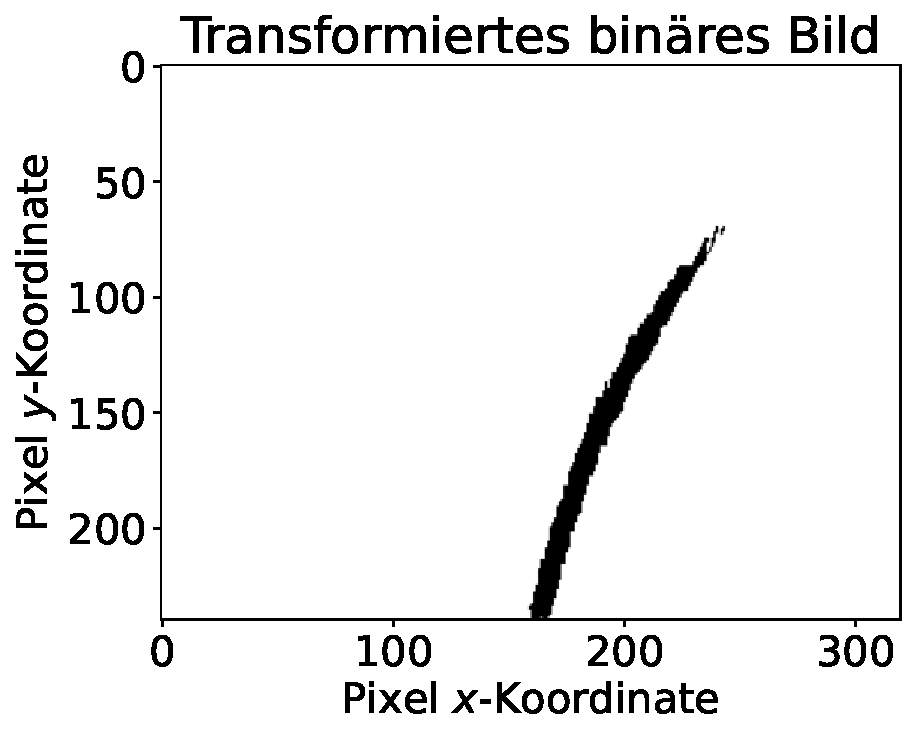
\includegraphics[scale=0.47]{hist1}
    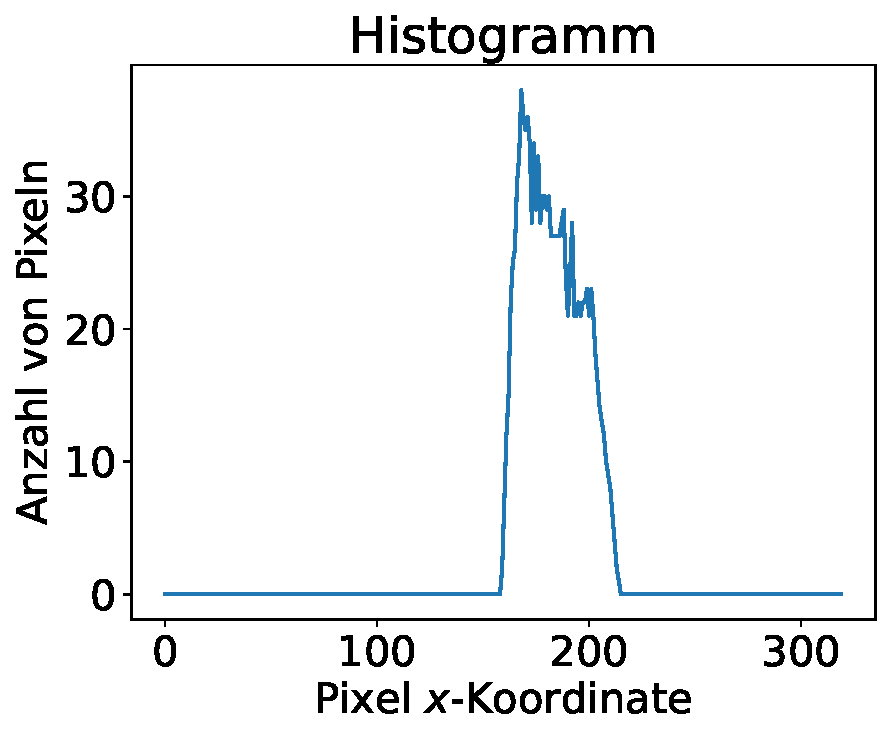
\includegraphics[scale=0.47]{hist2}
    \caption{Histogramm}
    \label{hist}
\end{figure}

\section{Gleitfenstermethode}

In der fünften Stufe der Pipeline wird es erstmal die Form der Spur bestimmt werden die Richtung und der Versatz (?) der
Fahrspur mit Hilfe der Gleitfenstermethode berechnet.

Zunächst wird eine ausgewählte Anzahl von Rechtecken (Fenstern) erstellt. Die
Fenster werden in einer Spalte ausgerichtet und sind gleich groß. Ihre Höhe
wird so gewählt, dass die Spalte die gesamte Höhe des Bildes überspannt,
während ihre Breite um einen Faktor der Bildbreite gewählt wird. Die Anzahl der
Fenster wird so gewählt, dass die Spalte die schwarzen Pixel umfasst, die die
Fahrspur darstellen, (?) wie in Abb. \ref{gleit} zu sehen ist. Wenn die Anzahl der
Fenster zu groß ist, besteht die Gefahr, dass die Methode weiße Pixel, die tief
im Bild liegen, fälschlicherweise als Teil der Fahrspur erkennt. 

Zweitens wird die x-Koordinate des Mittelpunkts des ersten Fensters auf den
Spitzenwert des Histogramms aus der vorherigen Stufe gesetzt. Dann wird die
Anzahl der weißen Pixel innerhalb des Fensters gezählt. Wenn die Anzahl über
einem gewählten Schwellenwert liegt, werden die Pixel zu einem Array
hinzugefügt und der Mittelwert der x-Koordinaten der enthaltenen Pixel
berechnet. (?) Die x-Koordinate des nächsten Fensters wird auf diesen
berechneten Mittelwert gesetzt und über das erste Fenster gelegt. Dieser
Vorgang wird dann für alle verbleibenden Fenster wiederholt. Wenn in einem
Fenster keine Pixel enthalten sind, wird das Fenster ignoriert und das folgende
Fenster darüber gelegt.  

Die Pixel, die nicht innerhalb der einzelnen Fenster liegen, werden dann aus
dem Bild herausgefiltert. Das Bild vor und nach dem Filterungsprozess ist in
Abb. \ref{gleit} zu sehen. Mit Hilfe der Methode der kleinsten Quadrate wird ein
Polynom durch die verbleibenden Pixel approximiert.

\begin{figure}[h]
    \centering
    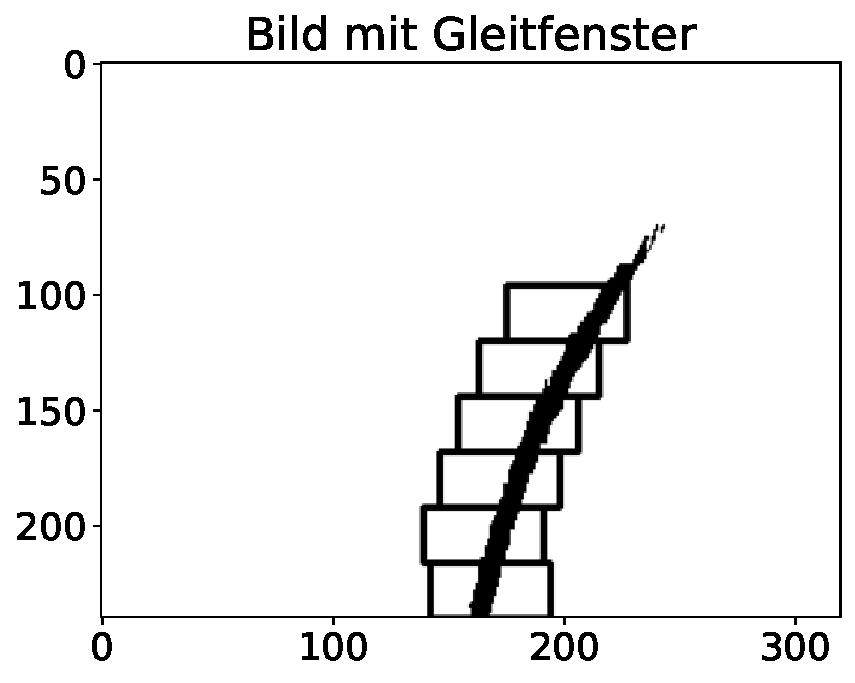
\includegraphics[scale=0.47]{before_filter}
    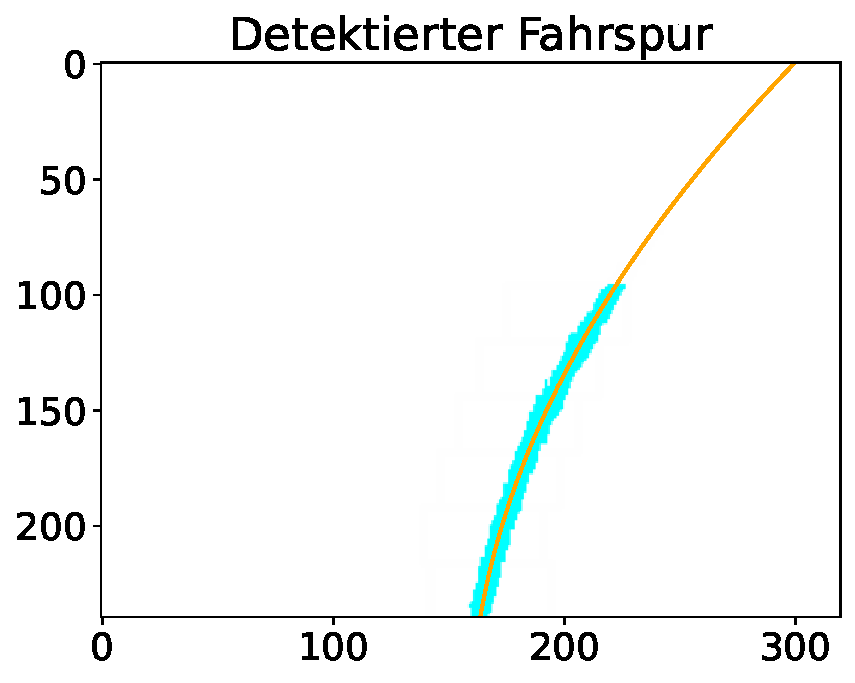
\includegraphics[scale=0.47]{after_filter}
    \caption{Vor und Nach dem Filterungsprozess}
    \label{gleit}
\end{figure}

\section{Berechnung von Ausrichtung und Abstand}

In dem letzten Schritt der Pipeline werden die Ausrichtung des Fahrzeugs und die Abweichung von
der Fahrspurlinie berechnet. 

Aus dem in der vorangegangenen Stufe berechneten Polynom wird eine
analytische Ausrichtung an einem ausgewählten Punkt entlang der Bahn mit der
folgenden Gleichung ermittelt, 
\begin{equation} 
    \theta = \arctan(f^\prime(y)).
\end{equation} 
Der arcus Tangens der Ableitung des Polynoms liefert die
Ausrichtung der Spur an einem bestimmten Punkt. Für den Stanley-Regler wird nur die
Differenz zwischen der Bahnausrichtung und der Ausrichtung des Fahrzeugs
benötigt, da es kein globales Koordinatensystem für das Fahrzeug gibt; die
Ausrichtung des Fahrzeugs wird so gewählt, dass sie zu jeder Zeit null Grad
beträgt. In Abb. \ref{ausrichtung} ist das Koordinatensystem des Fahrzeugs
dargestellt. 

\begin{figure}[h]
    \centering
    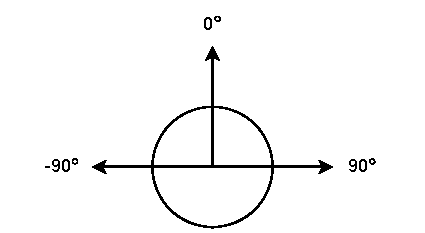
\includegraphics{fov}
    \caption{FOV}
    \label{ausrichtung}
\end{figure}

\iffalse
Der klassische Stanley-Regler, wie in Kapitel 2 beschrieben, verwendet die vom
nächstgelegenen Bahnpunkt berechnete Ausrichtung. Als Nebeneffekt der
Polynomanpassung ist jedoch die am unteren Bildrand berechnete Ausrichtung
falsch. Wie in ABBILDUNG zu sehen ist, kann die Gleitfenstermethode die
Fahrspurlinie in der Nähe des unteren Bildrandes nicht konsistent erkennen. Aus
diesem Grund wird die Ausrichtung durch das angepasste Polynom falsch
approximiert. Daher wird die Ausrichtung stattdessen an einem Punkt innerhalb
der erkannten Fahrspurlinie berechnet. Außerdem wird dadurch ein zusätzlicher
Freiheitsgrad für den Regler geschaffen. Die Konsequenzen daraus werden in
Kapitel 4 erörtert.
\fi

Die Abweichung von der Fahrspurlinie wird aus dem angepassten Polynom mit
folgender Funktion berechnet: 
\begin{equation}
    e_{V} = (\frac{w}{2} - f(h))\cdot x_{mpp}.
\end{equation}
Dabei ist $w$ die Breite des Bildes, $f(h)$ die Ausgabe des berechneten
Polynoms am unteren Rand des Bildes, $x_{mpp}$ eine Skalierungskonstante zur
Umrechnung von Pixeln in Meter und $e_{V}$ der Abstand des Fahrzeugs zur
Fahrspur. Zusammenfassend wird die Differenz aus der x-Komponente des
Mittelpunkts und der x-Komponente des Polynompunkts am unteren Bildrand in
Meter umgerechnet.

\section{Ausrei{\ss}er}

Die in Algorithmen zur Fahrspurerkennung verwendete Gleitfenstermethode kann zu
einem Phänomen führen, das als \glqq Ausreißer\grqq bekannt ist. Diese treten auf, wenn
der Algorithmus die Fahrspurlinie in einem bestimmten Bild falsch bestimmt.
Abb. \ref{ausrei} zeigt eine Sequenz von drei Einzelbildern, wobei das erste linke
Einzelbild den Ausgangspunkt bildet. Im ersten Bild wird die Fahrspurlinie
richtig erkannt, aber im zweiten Bild tritt ein Ausreißer auf, bei dem die
Fahrspurlinie falsch bestimmt wird. Im letzten Bild wird die Fahrspurlinie
wieder korrekt erkannt.

\begin{figure}[h]
    \centering
    \fbox{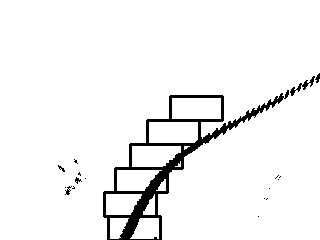
\includegraphics[scale=0.8]{before_outlier}}
    \fbox{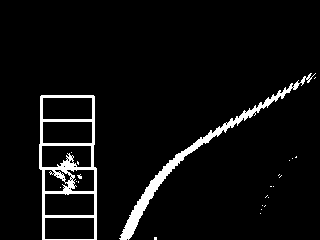
\includegraphics[scale=0.8]{outlier}}
    \fbox{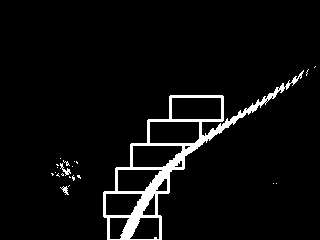
\includegraphics[scale=0.8]{after_outlier}}
    \caption{Ausrei{\ss}er}
    \label{ausrei}
\end{figure}

Eine der Hauptursachen für Ausreißer ist die falsche Auswahl der HSV-Werte im Color-Thresholding-Schritt.
Wenn die im Algorithmus verwendeten HSV-Werte nicht restriktiv genug sind,
werden Farben außer Gelb möglicherweise nicht herausgefiltert, was zu einer
ungenauen Bestimmung der Fahrspurlinie führt.


\section{Pipeline-Optimierungen}

Bei der Entwicklung der Bildverarbeitungspipeline wurde festgestellt, dass die
Laufzeit der Pipeline zu gro{\ss} war. Um die Rechenzeit der Pipeline auf ein
akzeptables Niveau zu verbessern, wurde eine Optimierung eingeführt. Weitere
Optimierungen sind zwar möglich, würden aber den Rahmen der Arbeit sprengen und
werden daher hier nicht behandelt.

Das Python-Programm cProfiler wurde verwendet, um die Funktionsaufrufe der
Pipeline mit ihren jeweiligen Laufzeiten zu untersuchen. Da es sich bei der
Pipeline um ein deterministisches Programm handelt, verbessert die
Zwischenspeicherung der Ausgabe der teuren Funktionsaufrufe im Speicher die
Laufzeit der Pipeline. Daher wird bei allen nachfolgenden Pipeline-Ausführungen
das zwischengespeicherte Ergebnis zurückgegeben, anstatt die Berechnung erneut
auszuführen. Beispielsweise ist die Berechnung der perspektivischen
Transformationsmatrizen kostspielig, was bei der Zwischenspeicherung zu einer
Leistungssteigerung der Pipeline führt.

FOR PAUL: 
This next paragraph exists in the english version, but I removed it here as it
no longer accurate due to our use of the corola brain.
Do you think I should still have it?


In order to prove the performance improvement of the pipeline, an experiment
was implemented. First, the pipeline is executed once and the runtime ignored
as the performance improvement is only relevant to subsequent executions of the
pipeline. Therefore, on the second execution of the pipeline, the runtime is
measured for both pipeline variants, with and without caching the expensive
function calls from the first execution. The experiment is then run 100 times
and the result tabulated. The arithmetic mean of the runtimes for both variants
are then compared to one another to measure the speed improvement. The values
are in TABLE, showing that by caching the expensive function calls, the
pipeline processing speed improved by VALUE%.


\chapter{Experiment}
\section{Hardware}

Die CoRoLa-Car-Platform besteht aus einem Raspberry Pi, einer Fisheye-Kamera,
einem b"urstenlosen Gleichstrommotor und einem Motorregler zur Steuerung der
Fahrzeuggeschwindigkeit und einem Servomotor um den Radeinschlag des Fahrzeugs
zu steuern. Der Raspberry Pi sendet PWM (Power-Werte) Signale an den Motorregler und den
Servoregler, um das Fahrzeug zu steuern. 

\section{Experimentkriterien}

\subsection{H"ochstgeschwindigkeit}

Um die Höchstgeschwindigkeit zu messen, fährt das Fahrzeug mit einer bestimmten
Vorwärtsgeschwindigkeit auf der Strecke. Wenn das Verhalten des Fahrzeugs als
\glqq akzeptabel\grqq angesehen wird, wird das Fahrzeug angehalten und die
Geschwindigkeit erhöht. Dieser Vorgang wird so lange wiederholt, bis das
Verhalten des Fahrzeugs nicht mehr \glqq akzeptabel\grqq ist. Das \glqq
akzeptable\grqq Verhalten des Fahrzeugs wird empirisch anhand der folgenden
beiden Kriterien definiert: Fähigkeit, der Fahrspur zu folgen, und Fehlen von
beobachteten Schwingungen.

\subsection{Maximal m"oglicher Fehlerwinkel}

Die maximalen Fehlerwinkel sind definiert als die maximalen Winkel, bei denen
das Fahrzeug in der Lage ist, den Weg links bzw. rechts der Fahrspurlinie
wiederzufinden. Um dies zu messen, wird das Fahrzeug bei deaktiviertem
Motorregler kollinear mit der Fahrspurlinie platziert. Dann wird das Fahrzeug
im Uhrzeigersinn gedreht, wobei der Ausgang des jeweiligen Reglers in Echtzeit
angezeigt wird. Das Fahrzeug wird so lange gedreht, bis der Ausgang des Reglers
entweder chaotisch wird oder konstant Null ist. Das Auftreten eines
chaotischen Ausgangs ist nicht deterministisch, empirisch gesehen ist dies
jedoch der Fall, wenn das Fahrzeug die Fahrspurlinie nicht zuverlässig erkennen
kann. Ein Ausgang von Null bedeutet auch, dass das Fahrzeug die Fahrspurlinie
überhaupt nicht erkennen kann.

\subsection{Abstand von der Linie}

Die Messung des Fahrzeugversatzes erfolgt durch die folgenden zwei Versuche.
Zunächst fährt das Fahrzeug mit einer bestimmten Vorwärtsgeschwindigkeit auf
der Strecke. Dann wird mit einer Überwachungskamera ein Video von der
Kurvenfahrt des Fahrzeugs aus der Vogelperspektive aufgenommen. Das Fahrzeug
wird mit unterschiedlichen Vorwärtsgeschwindigkeiten aufgezeichnet. Bei der
ersten Aufnahmerunde wird das Fahrzeug mit dem Stanley-Regler gesteuert, bei
der zweiten mit dem PID-Regler. Dieses Experiment wird für die gewählten
Geschwindigkeiten von 1,0, 1,25, 1,5, 1,75 und 2,0 Metern pro Sekunde
durchgeführt.

\subsection{Reglerausgang}

Um den Reglerausgang der beiden Regler zu messen, wird das Fahrzeug angewiesen
(?), mindestens dreimal um die Strecke zu fahren. Während der Fahrt wird der
Ausgang des Reglers aufgenommen. Nach der Fahrt werden die Daten im Zeitverlauf
grafisch dargestellt und eine Teilmenge der Daten ausgewählt. Die Teilmenge der
Daten wird nach den folgenden Kriterien ausgewählt: Periodizität und Fehlen von
Ausreißern.

\section{Ergebnisse}


\subsection{H"ochstgeschwindigkeit}
\begin{center}
\begin{tabular}{|c|c|}
\hline
    PID & Stanley \\
\hline
\hline
    1,5 m/s & 2,3 m/s \\
\hline
\end{tabular}
\end{center}
When running the PID controller on the vehicle, velocities above 1,5
$m/s$lead to issues with the robustness of the vehicle. In comparison
to then Stanley controller, whenever an outlier appears, the PID controller
causes the vehicle to oscillate and requires a longer time than the Stanley
controller to return to the lane. The oscillations scale with the forward
velocity of the vehicle. With velocities greater than or equal to 2,0
$m/s$, the PID controller will drive the vehicle into the wall of the
track. Even velocities between 1,5 and 1,75 $m/s$ require supervision
in order to make sure that the vehicle won't drive into the wall.

In comparsion, the Stanley controller requires no supervision, until the
forward velocity of the vehicle is above 2,3 $m/s$ However, at higher
velocities, the vehicle will drift farther from the path, until the vehicle
acts as a "guide", as opposed to something that needs to be followed. 

\subsection{Maximal m"oglicher Fehlerwinkel}


\begin{center}
\begin{tabular}{|c|c|c|}

\hline
    & PID (\textdegree) & Stanley (\textdegree)\\
\hline
\hline
    Uhrzeigersinn & 75 \pm 1& 50 \pm 1 \\
\hline
    Gegenuhrzeigersinn & 54 \pm 1 & 44 \pm 1 \\
\hline
\end{tabular}
\end{center}
The Stanley controller can not be offset from the lane as much as the PID
controller. Due to both the calibration stage of the pipeline and requiring an
approximated polynomial, the requirements for the Stanley controller to detect
the lane are higher than the PID controller. The PID controller requires only
that a grouping of yellow pixels exists in the image. The Stanley controller
requires at least some geometry to the grouping of yellow pixels, typically in
the form of a line or section of a curve.

\subsection{Abstand von der Linie}

As can be seen in FIGURE, the PID controller follows the path closer than the
Stanley controller. Even accounting for the offset at the start of the curve,
the Stanley controller does not drive the vehicle onto the lane until the end
of the curve. In comparison, the PID controller forces the vehicle to stay on
the path, while still drifting lightly to the left. This drift scales with the
forward velocity of the vehicle.

When comparing the results of the simulation of the Stanley controller in
FIGURE with $v = 1,75 m/s$ and $fs = 50$ Hz and its behaviour on the
track, the behaviour of the Stanley controller in reality matches with the
simulation. However, as can be seen in FIGURE, the Stanley controller will
drift away from the straight section of the track before the curve. 

Compensation for this drift was attempted, but outside of setting the reference
point for the cross-track-error to another value, the drift stayed. By changing
the reference point manually, the vehicle requires different parameters when
driving clockwise or counterclockwise around the track. To avoid this, it was
decided to keep the drift included for now. In chapter 5, adjustments to the
Stanley controller are discussed, that could lead to an improvement in the
future.

\begin{figure}[h]
    \centering
    \fbox{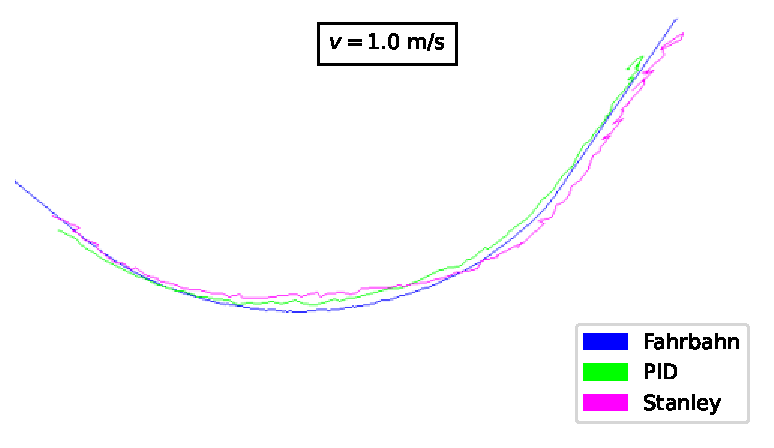
\includegraphics[scale=0.8]{done1.0}}
    \caption{1.0}
    \label{ausrei}
\end{figure}

\begin{figure}[h]
    \centering
    \fbox{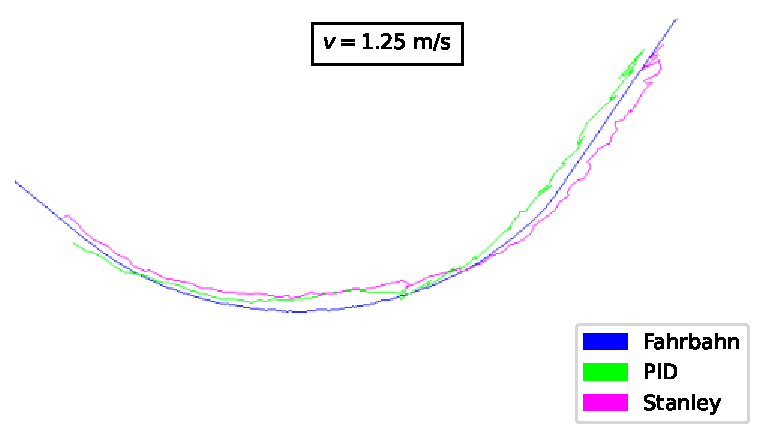
\includegraphics[scale=0.8]{done1.25}}
    \caption{1.25}
    \label{ausrei}
\end{figure}
\begin{figure}[h]
    \centering
    \fbox{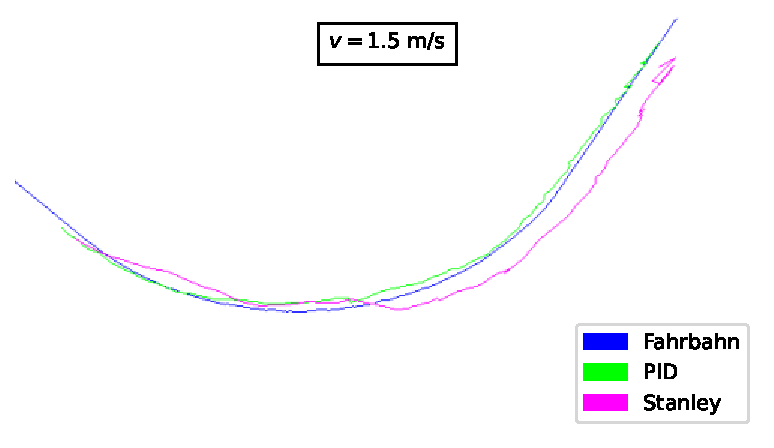
\includegraphics[scale=0.8]{done1.5}}
    \caption{1.5}
    \label{ausrei}
\end{figure}
\begin{figure}[h]
    \centering
    \fbox{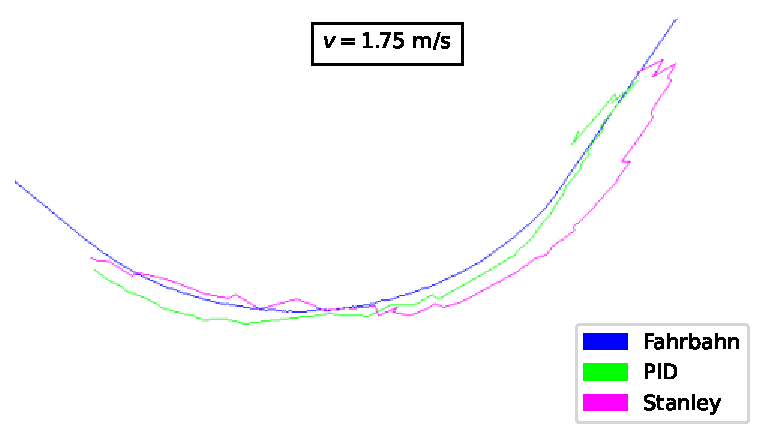
\includegraphics[scale=0.8]{done1.75}}
    \caption{1.75}
    \label{ausrei}
\end{figure}
\begin{figure}[h]
    \centering
    \fbox{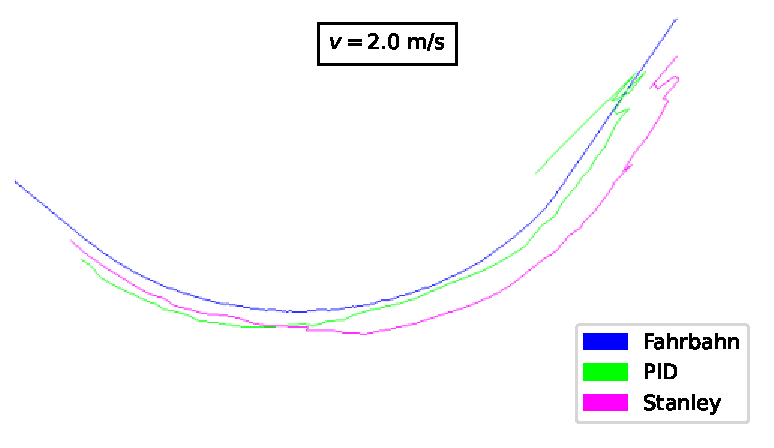
\includegraphics[scale=0.8]{done2.0}}
    \caption{2.0}
    \label{ausrei}
\end{figure}
\subsection{Reglerausgang}

\begin{center}
\begin{tabular}{|c|c|c|}
\hline
    Geschwindigkeit (m/s) & PID (\textdegree) & Stanley (\textdegree)\\
\hline
\hline
    1,0 & 5,33 & 4,79 \\ 
\hline
    1,25 & 11,97 & 11,82 \\
\hline
    1,5 & 9,61 & 13,19 \\
\hline
    1,75 & 12,35 & 13,30 \\
\hline
    2,0 & 13,84 & 13,51 \\
\hline
\end{tabular}
\end{center}

The controller output of both controllers are similar, regardless of the
velocity, except for the PID controller at velocity 1,5 $m/s$. As the
forward velocity of the vehicle increases, the controller output scales
appropiately. The difference between the two controllers comes in the form of
both signals. Between forward velocities 1,0 and 1,5 $m/s$, the signal
output of the two controllers are similar, however at 1,75 and 2,0
$m/s$ the sinusoidal nature of the PID controller degrades, while the
sinusoidal nature of the Stanley controller increases. 

At 1,75 $m/s$ the PID controller can still control the vehicle onto
the lane, however as can be seen in FIGURE, outliers lead to high oscillations
in controller output. When the PID controller incorrectly identifies the lane,
the controller has difficulty returning the vehicle to the lane and can instead
drive the vehicle into the wall, which can be seen at the right end of the
graph. In comparison, the Stanley controller has no issue following the path at
the same velocity. 

At 2,0 $m/s$ the PID controller is unable to control the vehicle and
drives the vehicle into the wall. As can be seen in FIGURE, the output varies
between -30 and 30 degrees and there is no periodicity. In comparision, the
Stanley controller has a stable oscillation between -30 and 0 degrees and is
periodic.

Outliers do not lead to high oscillations when the vehicle is being controlled
by the Stanley controller. It has been observed that the vehicle will reorient
itself onto the path much quicker than the PID controller.

\begin{figure}[h]
    \centering
    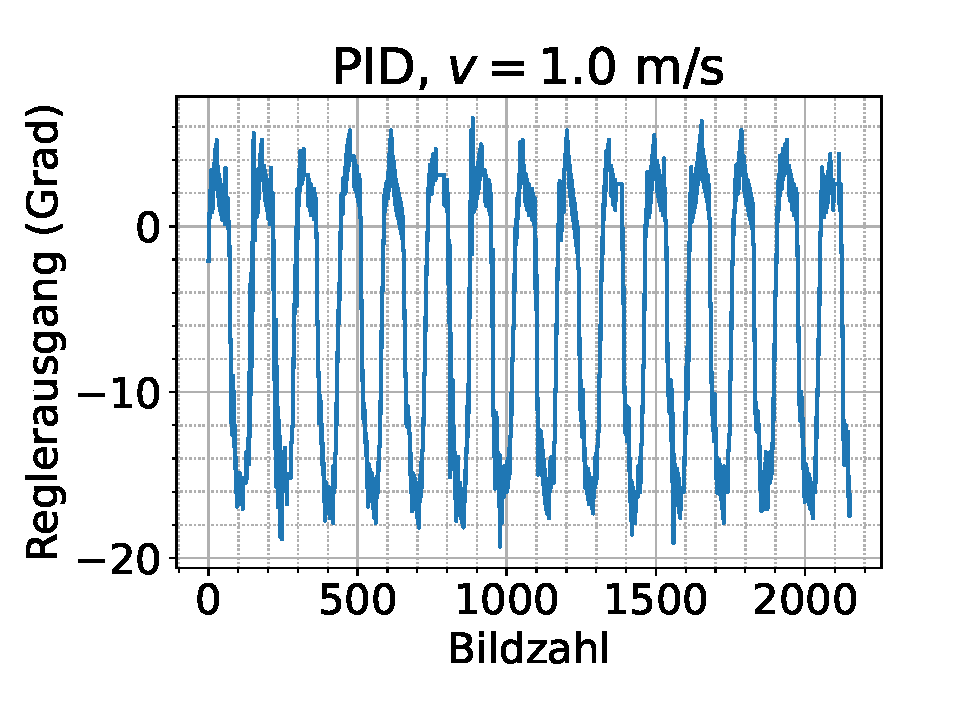
\includegraphics[scale=0.47]{pid1.0}
    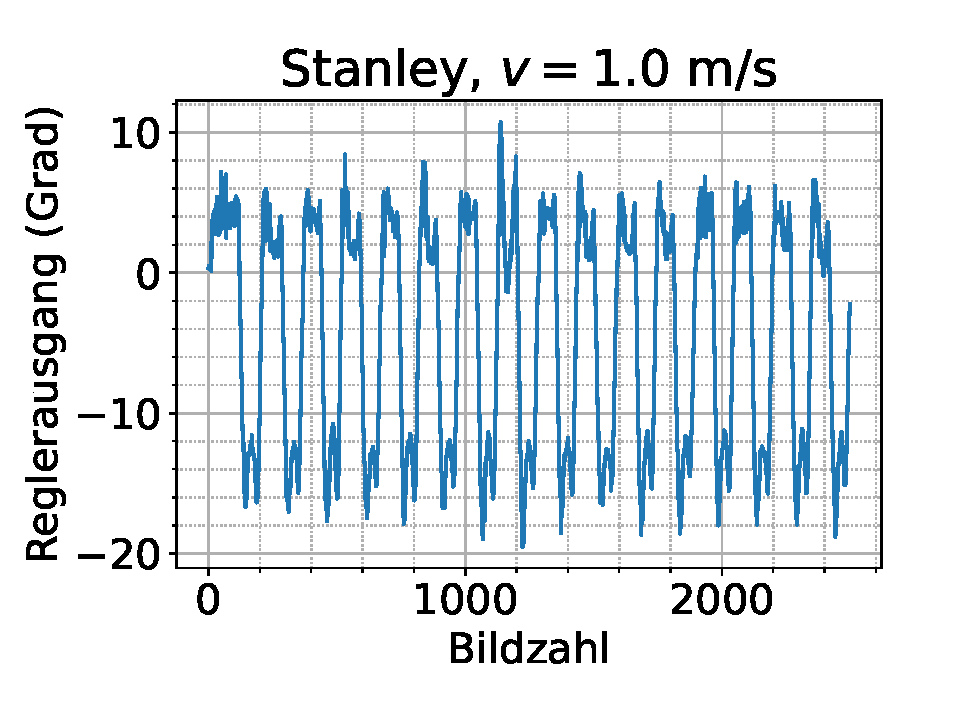
\includegraphics[scale=0.47]{Stan1.0}
    \caption{1.0}
    \label{ausrei}
\end{figure}

\begin{figure}[h]
    \centering
    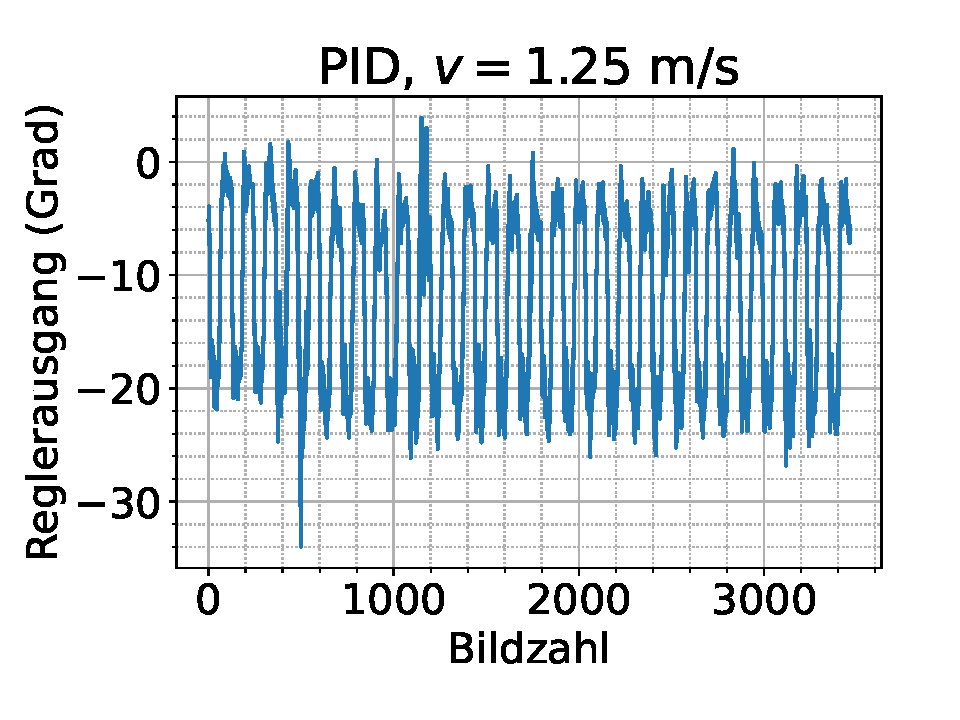
\includegraphics[scale=0.47]{pid1.25}
    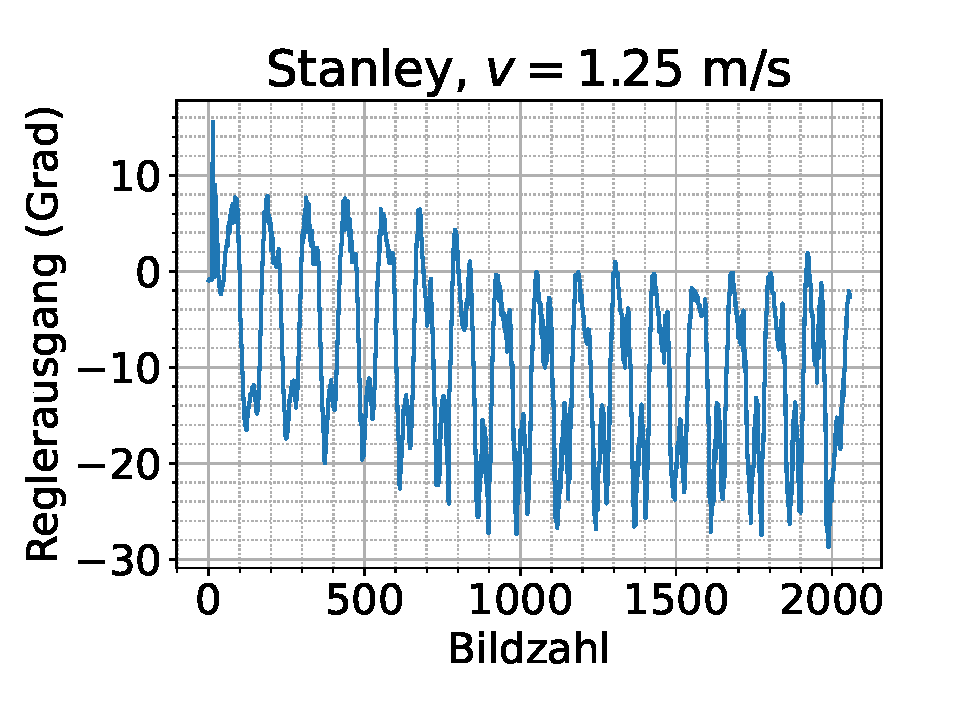
\includegraphics[scale=0.47]{Stan1.25}
    \caption{1.25}
    \label{ausrei}
\end{figure}

\begin{figure}[h]
    \centering
    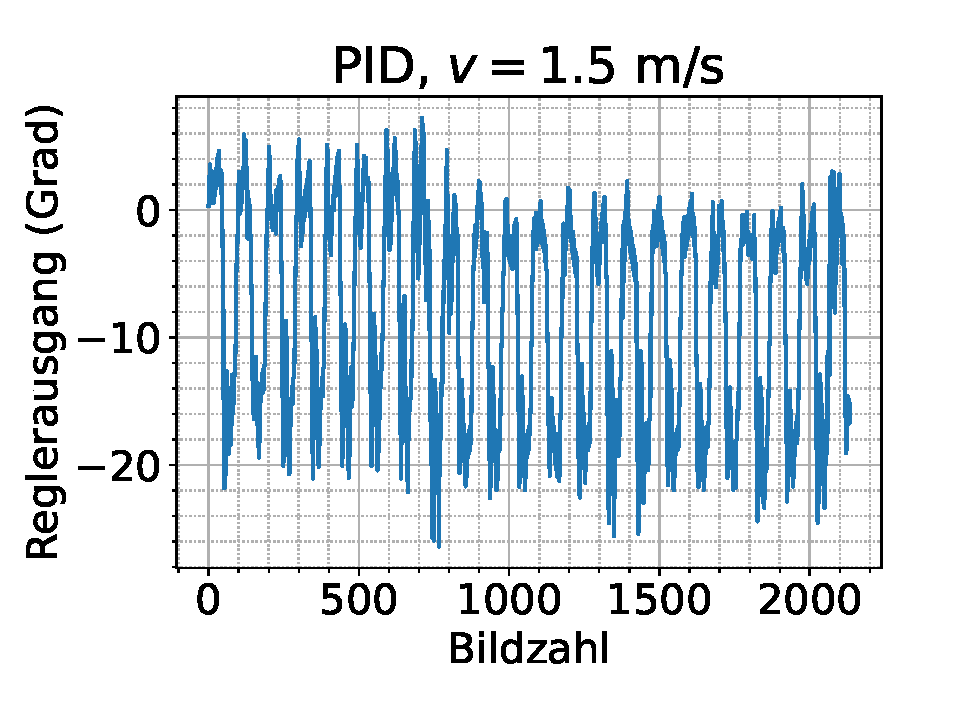
\includegraphics[scale=0.47]{pid1.5}
    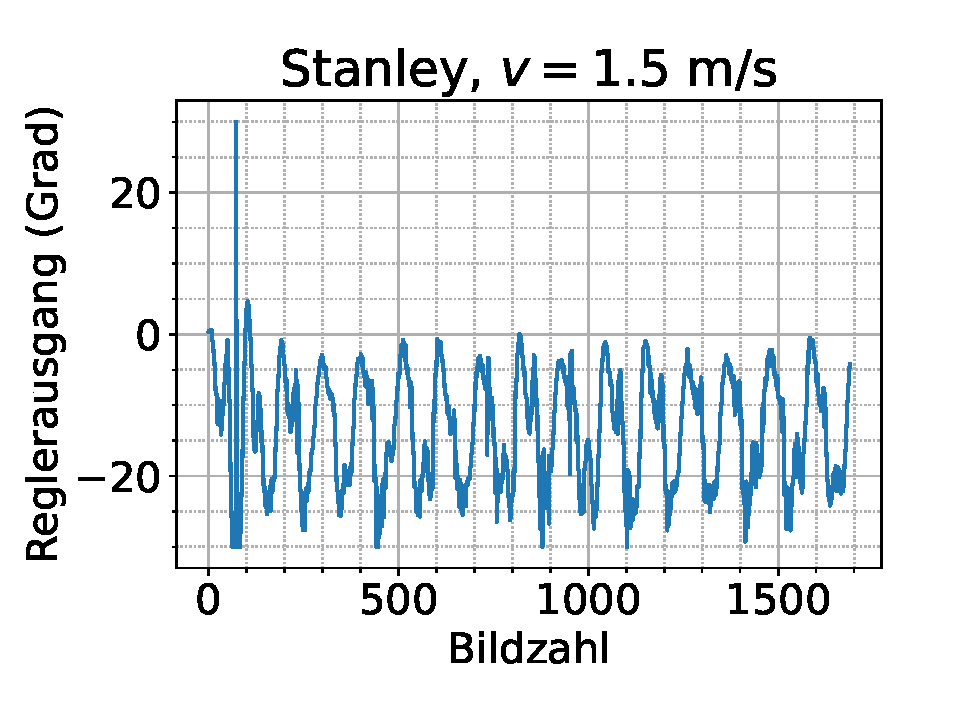
\includegraphics[scale=0.47]{Stan1.5}
    \caption{1.5}
    \label{ausrei}
\end{figure}

\begin{figure}[h]
    \centering
    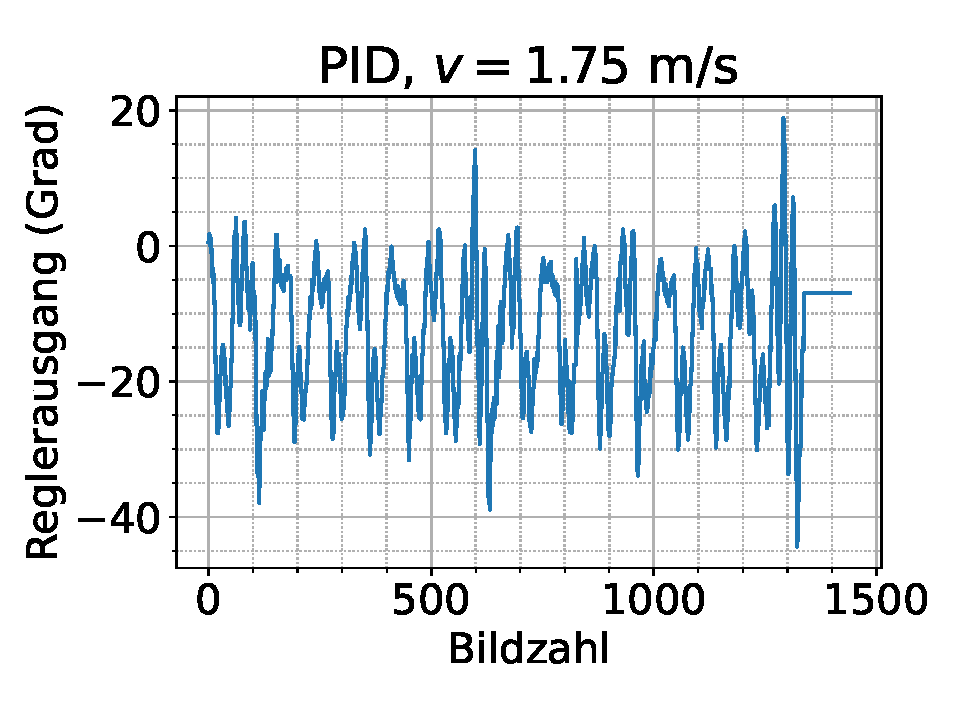
\includegraphics[scale=0.47]{pid1.75}
    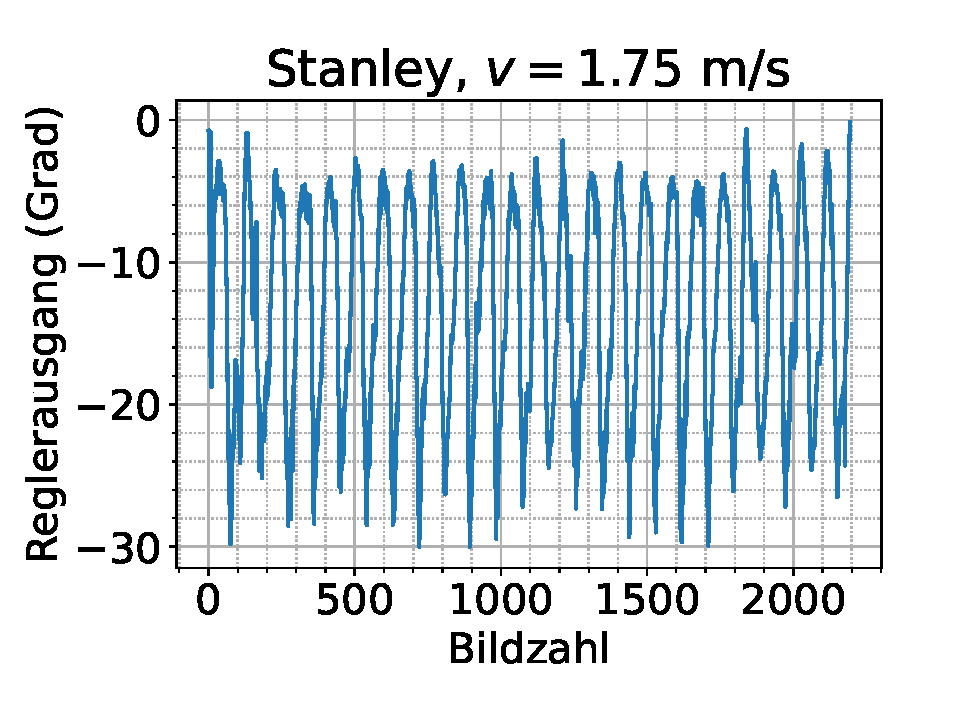
\includegraphics[scale=0.47]{Stan1.75}
    \caption{1.75}
    \label{ausrei}
\end{figure}

\begin{figure}[h]
    \centering
    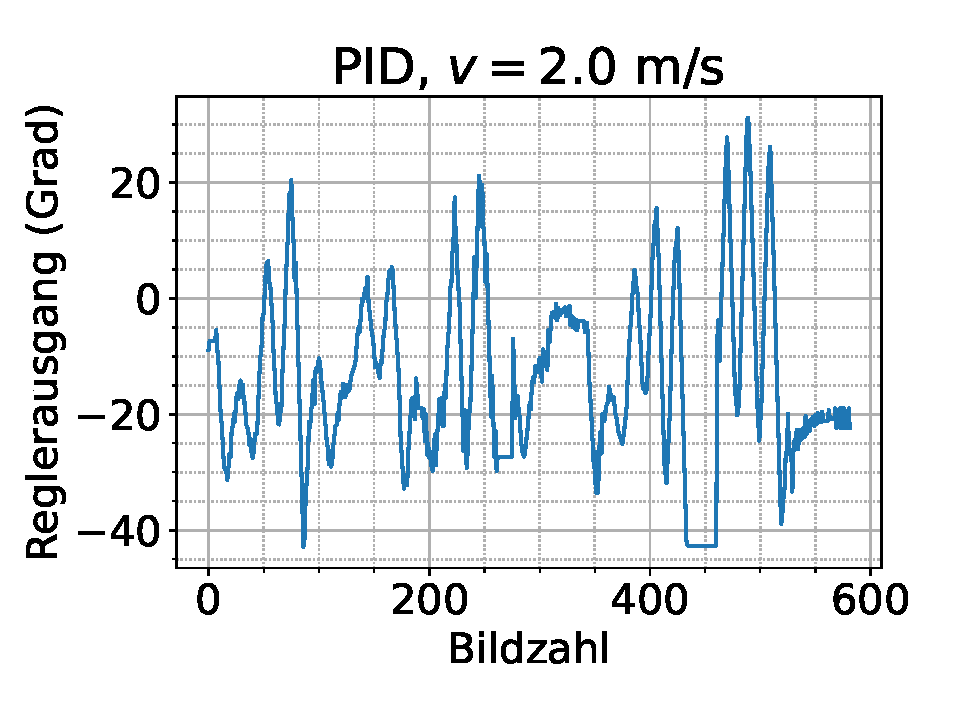
\includegraphics[scale=0.47]{pid2.0}
    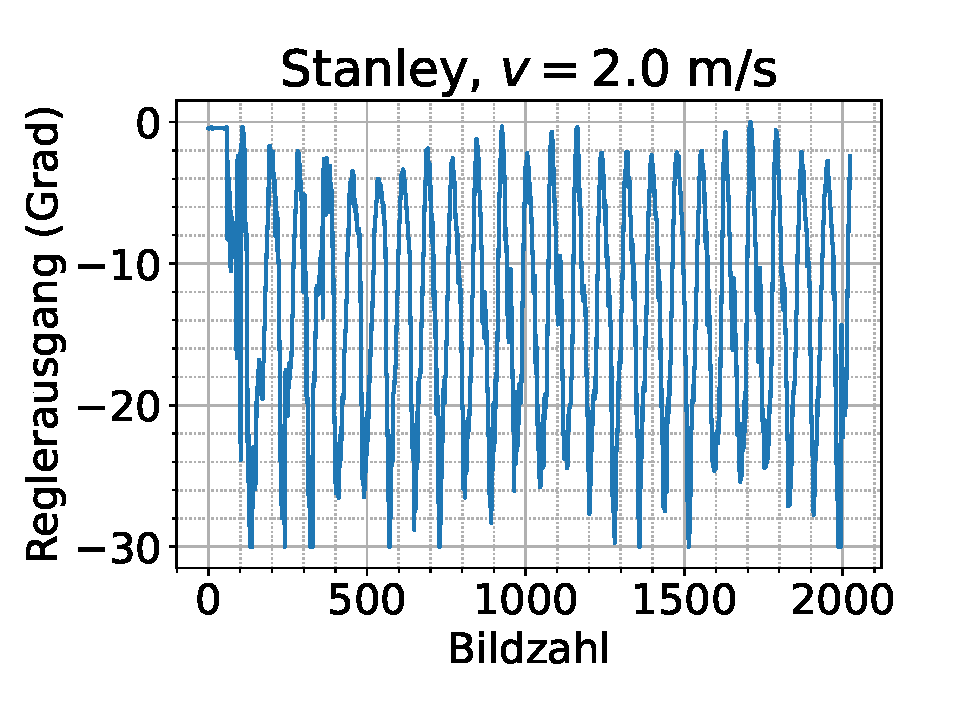
\includegraphics[scale=0.47]{Stan2.0}
    \caption{2.0}
    \label{ausrei}
\end{figure}




\chapter{Conclusion}


When comparing only the path following behaviour of both controllers, the PID
controller is still the best choice. However, when factoring in the other
aspects of the problem statement, the Stanley controller is a better fit for
the application. As the vehicle needs to be able to drive autonomously without
supervision at a higher velocity than it can originally, the Stanley controller
fulfills these requirements. 

\subsection{Future Work}

By the conclusion of this paper, the vehicle still drifts away from the
lane before each curve. In the future, it is proposed to adjust the Stanley
controller to include an integrator in order to compensate for this drift.
The adjusted Stanley controller has the form of the following equation:

\begin{equation} 
    u = \theta - \theta_d + \arctan\left(\frac{ke_{V}}{v}\right) + k_{i} \int_{0}^{t} e_{V}\,d\tau, 
    \label{eq:Stanley-Regler-adjusted} 
\end{equation}

In linear control theory, an integrator is used in order to remove residual
error from an application. As the small signal version of the Stanley
controller is a PD controller, it is hypothesized that an integrator will 
correct this observed drift. As can be seen in FIGURE, the drift is apparent in
the input to the controller. By integrating the offset it is proposed that
over time the drift will be componsated for and the vehicle stay on the lane. 

\end{document}
